\documentclass[12pt]{report}
\usepackage[english, magyar]{babel}
\usepackage{t1enc}
\frenchspacing

\usepackage[margin=2cm, top=5cm, bottom=2.5cm, bindingoffset=0cm]{geometry}
\usepackage{graphicx}

\usepackage{hyperref}
\hypersetup{hidelinks}

\usepackage{xcolor,listings}
\usepackage{textcomp}
\usepackage{color}
\usepackage{listingsutf8}

\definecolor{codegreen}{rgb}{0,0.6,0}
\definecolor{codegray}{rgb}{0.5,0.5,0.5}
\definecolor{codepurple}{HTML}{C42043}
\definecolor{backcolour}{HTML}{F2F2F2}
\definecolor{bookColor}{cmyk}{0,0,0,0.90}  
\color{bookColor}
\lstset{upquote=true}

\lstdefinestyle{mystyle}{  
	commentstyle=\color{codegreen},
	keywordstyle=\color{blue},
	numberstyle=\footnotesize\color{codegray},
	stringstyle=\color{codepurple},
	basicstyle=\footnotesize,
	breakatwhitespace=false,         
	breaklines=true,                 
	captionpos=b,                    
	keepspaces=true,                 
	numbers=left,                    
	numbersep=-10pt,                  
	showspaces=false,                
	showstringspaces=false,
	showtabs=false, 
	inputencoding = utf8,  % Input encoding
	extendedchars = true,  % Extended ASCII
	literate      =        % Support additional characters
	{á}{{\'a}}1  {é}{{\'e}}1  {í}{{\'i}}1 {ó}{{\'o}}1  {ú}{{\'u}}1
	{Á}{{\'A}}1  {É}{{\'E}}1  {Í}{{\'I}}1 {Ó}{{\'O}}1  {Ú}{{\'U}}1
	{à}{{\`a}}1  {è}{{\`e}}1  {ì}{{\`i}}1 {ò}{{\`o}}1  {ù}{{\`u}}1
	{À}{{\`A}}1  {È}{{\'E}}1  {Ì}{{\`I}}1 {Ò}{{\`O}}1  {Ù}{{\`U}}1
	{ä}{{\"a}}1  {ë}{{\"e}}1  {ï}{{\"i}}1 {ö}{{\"o}}1  {ü}{{\"u}}1
	{Ä}{{\"A}}1  {Ë}{{\"E}}1  {Ï}{{\"I}}1 {Ö}{{\"O}}1  {Ü}{{\"U}}1
	{â}{{\^a}}1  {ê}{{\^e}}1  {î}{{\^i}}1 {ô}{{\^o}}1  {û}{{\^u}}1
	{Â}{{\^A}}1  {Ê}{{\^E}}1  {Î}{{\^I}}1 {Ô}{{\^O}}1  {Û}{{\^U}}1
	{œ}{{\oe}}1  {Œ}{{\OE}}1  {æ}{{\ae}}1 {Æ}{{\AE}}1  {ß}{{\ss}}1
	{ç}{{\c c}}1 {Ç}{{\c C}}1 {ø}{{\o}}1  {Ø}{{\O}}1   {å}{{\r a}}1
	{Å}{{\r A}}1 {ã}{{\~a}}1  {õ}{{\~o}}1 {Ã}{{\~A}}1  {Õ}{{\~O}}1
	{ñ}{{\~n}}1  {Ñ}{{\~N}}1  {¿}{{?`}}1  {¡}{{!`}}1	{ő}{{\"O}}2
	{ű}{{\"U}}2
	{°}{{\textdegree}}1 {º}{{\textordmasculine}}1 {ª}{{\textordfeminine}}1
}
\lstset{style=mystyle} 

\usepackage{fancyhdr}
\fancypagestyle{plain}{
\fancyhf{}
\fancyhead[R]{\leftmark}
\fancyhead[L]{\thepage}
\fancyfoot[C]{Adatkezelés XML környezetben}}

\fancyhead[R]{\leftmark}
\fancyhead[L]{\thepage}
\fancyfoot[C]{Adatkezelés XML környezetben}

\begin{document}
	\pagestyle{fancy}
	\title{\Huge JEGYZŐKÖNYV \\ \LARGE Adatkezelés XML környezetben}
	\author{\Large Féléves feladat: Állatkerthálózat}
	\date{\vspace{250px}
		\begin{flushleft}
			Készítette: \textbf{Martinák Mátyás}\\
			Neptunkód: \textbf{KLNSPG}\\
			Dátum: \textbf{2023. 10. 25.}
		\end{flushleft}
		\vspace{15px}
		\begin{center}
			\textbf{Miskolc, 2023}
		\end{center}}
	\maketitle
	
\tableofcontents
\clearpage

\fancyhf{}
\fancyhead[L]{\thepage}

\chapter{A feladat leírása}
A feladat egy vagy több állatkert hálózatát mutatja be, amiben helyet kapnak az egyes állatkertekben dolgozók, azok feladatai, az állatok és élőhelyeik, eledelük, az eledelt gyártó cégek, illetve az állatok örökbefogadói, ha vannak. Mind az ER modell tervezésben és mind az XML megvalósításban angol nyelvet használtam, ugyanis ez a legelterjedtebb nyelv a programozásban\\
Összesen 6 egyedet hoztam létre, melyek a következők:
\begin{itemize}
	\item Employee,
	\item Site,
	\item Habitat,
	\item Animal,
	\item Food,
	\item User
\end{itemize}

\indent Legelőször is érdemes pár szót szólni a \textbf{Site} egyedről. Innen indul ki minden. Ez az egyed tárolja el az egyes
állatkertek legfőbb tulajdonságait, mint pl. név, terület vagy éppen nyitva tartás. Elsődleges kulcsa a \texttt{site\_id}, ami
az állatpark azonosítója.

A Site és az \textbf{Employee} egyed között egy \texttt{1:N} kapcsolat van, mivel egy állatkerthez több dolgozó is tartozhat,
de egy dolgozó, csak egy állatkerthez tartozhat. Az \texttt{1:N} kapcsolat neve: \textbf{Works}. Egy dolgozónak van azonosítója,
vezeték és keresztneve (ami ER modellben egy többágú tulajdonság), neme, születési dátuma és ami a legfontosabb, a dolgozó feladatai, posztjai, amiből lehet egy vagy több, így ez egy többértékű tulajdonság lesz. Ez azért fontos, mivel a relációs modellnél ez a tulajdonság egy külön táblát kap majd, amiben lesz a posztnak egy id-ja, a poszt neve, illetve, hogy kihez tartozik.

Egy állatkerthez több élőhely is tartoztat, de egy élőhely csak egy állatkerthez tartozik. Ezt ábrázolja a \textbf{Manage} kapcsolat, ami \texttt{1:N} kapcsolattal köti össze a Site és a \textbf{Habitat} egyedeket. Az élőhelynek nincsenek ,,extra'' tulajdonságai, van egy azonosítója, neve, térképen való elhelyezkedése, leírása és kapacitása, hogy mennyi állatot
képes egyszerre befogadni.

Az \textbf{Occupy} kapcsolat szintén \texttt{1:N} kapcsolattal köti össze a Habitat-ot az \textbf{Animal}-lel. Az állatnak van azonosítója, neve, faja és leírása.

Itt jön a legelső \texttt{N:M} kapcsolat, az \textbf{Eat}, aminek lesz tulajdonsága, a \texttt{feeding\_time}, az etetési idő. Fontos, hogy megjegyezzük, az \texttt{N:M} kapcsolat külön kapcsolótáblát fog kapni a relációs modellben. Az Eat köti össze az Animalt
a \textbf{Food}-dal, ami az állat eledelét modellező egyed. Ennek van azonosítója, neve, egy \texttt{boolean} (logikai) értéke, ami azt dönti el, hogy finom-e az adott eledel, vagy sem. Ezen kívül van egy többértékű tulajdonsága is, az eledeleket gyártó cégek, amik szintén külön táblát fognak majd kapni a relációs modellben.

Az állatokat örökbe is lehet fogani bizonyos \textbf{User}-eknek, ezt a \textbf{Favor} \texttt{1:1} kapcsolat modellezi. Talán a Usernek
van a legtöbb tulajdonsága ebben az adatbázisban. Van természetesen azonosítója, két neve (vezeték és keresztnév), neme, bejelentkezési adatai (felhasználónév, jelszó), mivel online szeretnénk lebonyolítani az állatok örökbefogadását. Ezen kívül címe is van a felhasználónak, ami az irányítószám, város, utca, házszám tulajdonságokból tevődik össze.

\chapter{I. feladat - XML/XSD létrehozás}

\section[ER modell]{A feladat ER modellje}

\begin{figure}[h]
	\centering
	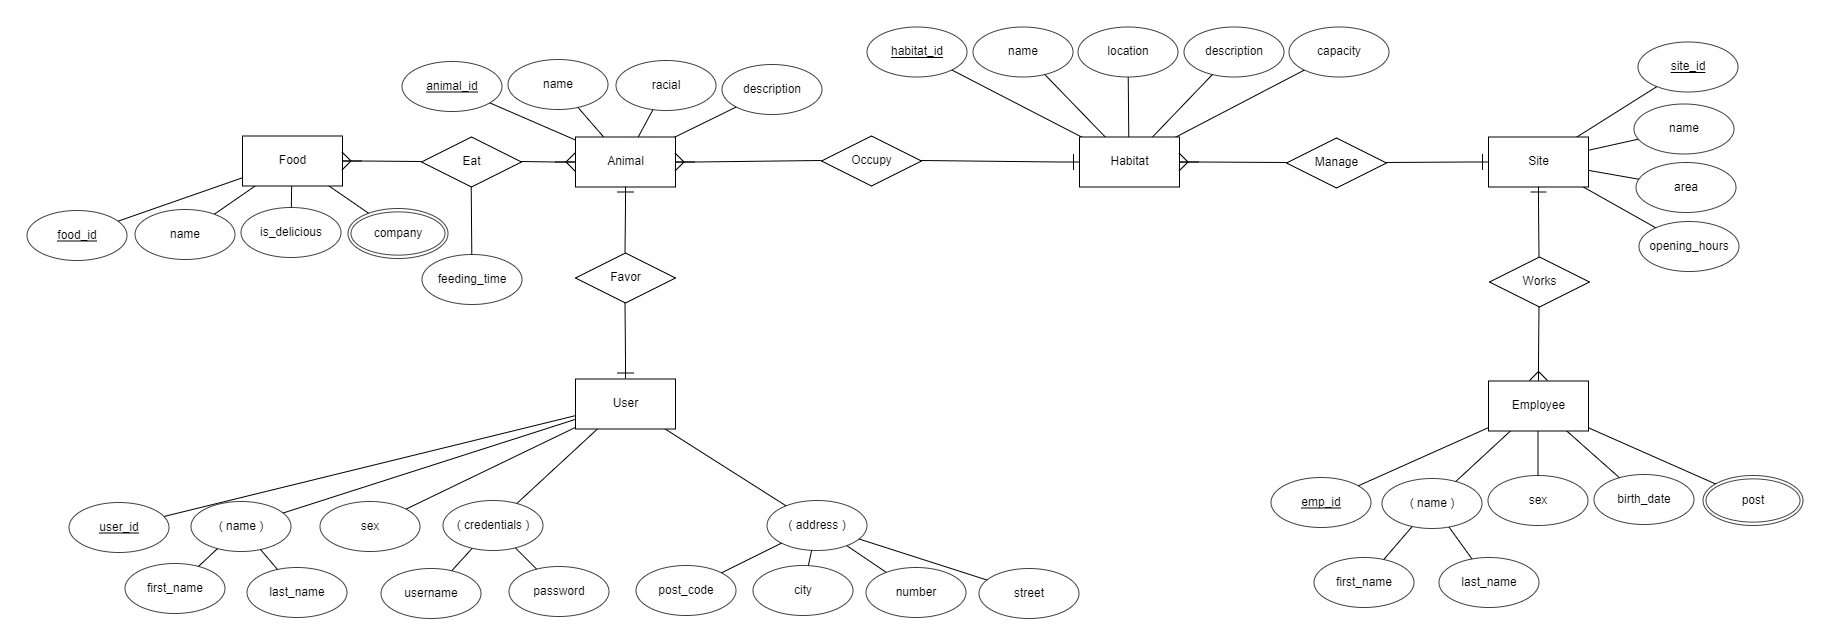
\includegraphics[width=0.999\linewidth]{ERKLNSPG.png}
	\caption{A feladat ER modellje}
\end{figure}

\section[XDM modell]{A feladat XDM modellje}

\indent\indent A konvertáláskor figyelembe kell venni az ER modell során definiált kapcsolatokat, azok típusait (\texttt{1:1, 1:N, N:M}), illetve az entitások elsődleges kulcsait is. Minden \textit{egy-több} kapcsolat esetében ahhoz az elsődleges kulcshoz kerül a szaggatott nyíl, ahol az ER modellben a ,,több'' szerepel. Az ,,Eat'' és a ,,Favor'' kapcsolatokat kivéve, mindenhol \texttt{1:N} kapcsolat szerepel az ER modellben, így az XDM mindenhol majdnem hasonlóan fog kinézni. Az \texttt{N:M} kapcsolat esetében egy új modellt veszünk fel, tulajdonsággal és \textit{primary key}-el együtt természetesen, ahonnan a nyilakat a fő entitásokhoz húzzuk. A többágú tulajdonságok itt is több tulajdonsággal rendelkeznek, a többértékű tulajdonságok itt nem kapnak külön modellt. Az XDM modell gyökéreleme: \textbf{Zoo\_KLNSPG}

\begin{figure}[h]
	\centering
	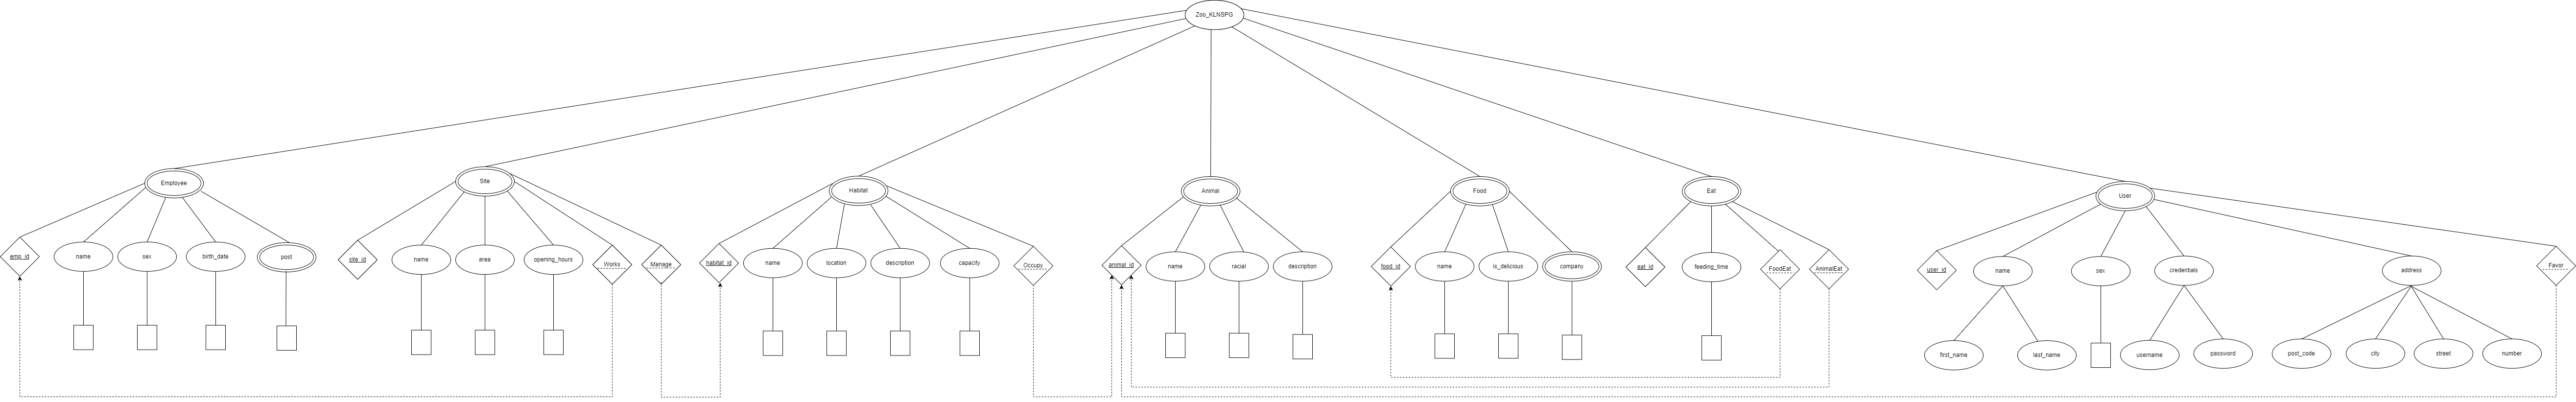
\includegraphics[width=1.01\linewidth]{XDMKLNSPG.png}
	\caption{A feladat XDM modellje}
\end{figure}

A ,,Works'' kapcsolat \texttt{1:N}, ahol a több érték az \textit{Employee}-hoz kerül, így a kapcsolatot is az \textit{emp\_id}-hez húzzuk. Szintén ugyan ez a helyzet a ,,Manage'' kapcsolatnál is, ahol a rombuszt a \textit{habitat\_id}-hoz húzzuk. Az \textit{Animal} modell egy különleges, ide 3 kapcsolatot is húzunk, melyek:

\begin{itemize}
	\item ,,Manage'' a \textit{Habitat}-ból
	\item ,,AnimalEat'' az \textit{Eat}-ből és végül
	\item ,,Favor'' a \textit{User}-ből 
\end{itemize}
Kettő \texttt{1:N} kapcsolat és egy \texttt{1:1} kapcsolat húz ide.

\section{Az XDM modell alapján XML dokumentum készítése}
\section{Az XML dokumentum alapján XMLSchema készítése}
\chapter{II. feladat - DOM}
\section{Adatolvasás}
\section{Adatmódosítás}
\section{Adatlekérdezés}
\section{Adatírás}

\end{document}